\documentclass{article}
\usepackage[utf8]{inputenc}
\usepackage{amsmath}
\usepackage{graphicx}
\usepackage{hyperref}
\usepackage{booktabs} % Para tablas con mejor formato
\usepackage{float} % Para controlar la posición de las figuras

\begin{document}

\section{Pruebas Iniciales y Resultados Preliminares (30\%)}

\subsection{a) Descripción}

Esta sección detalla las pruebas iniciales realizadas sobre el modelo de detección entrenado, con el objetivo de validar los aspectos fundamentales de su diseño e identificar áreas que requieren ajustes o mejoras. Se presenta un análisis exhaustivo de las métricas de rendimiento obtenidas durante el proceso de entrenamiento, lo que permite una evaluación crítica de la capacidad del modelo para detectar objetos de interés en el conjunto de datos de validación.

\subsection{b) Evidencias Esperadas}

Los resultados del entrenamiento del modelo de detección, generados en la ruta \texttt{DATASETS/runs/detect/train}, proporcionan una visión detallada de su rendimiento. A continuación, se presentan las métricas clave y un análisis de los resultados, demostrando cómo esta información ha guiado ajustes en el diseño e implementación del modelo.

\textbf{Configuración del Entrenamiento (extraído de \texttt{DATASETS/runs/detect/train/args.yaml}):}
\begin{itemize}
    \item \textbf{Modelo:} \texttt{yolov8n.pt}
    \item \textbf{Épocas:} 100
    \item \textbf{Tamaño de imagen:} 640
    \item \textbf{Batch Size:} 32
\end{itemize}

\textbf{Métricas de Rendimiento (última época, extraído de \texttt{DATASETS/runs/detect/train/results.csv}):}

\begin{table}[h!]
    \centering
    \begin{tabular}{lc}
        \toprule
        \textbf{Métrica} & \textbf{Valor (Época 100)} \\
        \midrule
        \texttt{metrics/precision(B)} & 0.99187 \\
        \texttt{metrics/recall(B)} & 0.98986 \\
        \texttt{metrics/mAP50(B)} & 0.99410 \\
        \texttt{metrics/mAP50-95(B)} & 0.99142 \\
        \texttt{train/box\_loss} & 0.15191 \\
        \texttt{train/cls\_loss} & 0.13024 \\
        \texttt{train/dfl\_loss} & 0.86309 \\
        \texttt{val/box\_loss} & 0.15189 \\
        \texttt{val/cls\_loss} & 0.12686 \\
        \texttt{val/dfl\_loss} & 0.77060 \\
        \bottomrule
    \end{tabular}
    \caption{Métricas de rendimiento del modelo en la última época de entrenamiento.}
    \label{tab:metrics}
\end{table}

\textbf{Análisis de Resultados:}

\begin{itemize}
    \item \textbf{Precisión (Precision) y Recall:} Los valores de precisión (0.99187) y recall (0.98986) en la última época son excepcionalmente altos, indicando que el modelo es muy bueno tanto en la identificación correcta de objetos como en la minimización de falsos positivos y falsos negativos. Esto sugiere que el modelo tiene una gran capacidad para distinguir entre las clases y localizar los objetos con exactitud.

    \item \textbf{F1-score:} Aunque no se proporciona directamente, con valores tan altos de precisión y recall, el F1-score (que es la media armónica de precisión y recall) también sería muy alto, confirmando un excelente equilibrio entre ambas métricas.

    \item \textbf{mAP (mean Average Precision):} El mAP50 (0.99410) y mAP50-95 (0.99142) son métricas cruciales que evalúan la precisión promedio en diferentes umbrales de IoU (Intersection over Union). Un mAP50 de casi 0.994 indica que el modelo es extremadamente preciso en la detección de objetos con un umbral de IoU del 50\%. El mAP50-95, que promedia el mAP en umbrales de IoU desde 50\% hasta 95\%, también es muy alto (0.99142), lo que demuestra la robustez del modelo incluso con requisitos de localización más estrictos.

    \item \textbf{Curvas de Pérdida (Loss Curves):} Las pérdidas de entrenamiento (\texttt{train/box\_loss}, \texttt{train/cls\_loss}, \texttt{train/dfl\_loss}) y de validación (\texttt{val/box\_loss}, \texttt{val/cls\_loss}, \texttt{val/dfl\_loss}) muestran una tendencia decreciente a lo largo de las épocas, lo que es un indicador positivo de que el modelo está aprendiendo y convergiendo. Los valores finales de pérdida son bajos, lo que sugiere que el modelo ha minimizado los errores de localización (box\_loss), clasificación (cls\_loss) y distribución de características (dfl\_loss). La cercanía entre las pérdidas de entrenamiento y validación al final del entrenamiento (por ejemplo, \texttt{train/box\_loss} 0.15191 vs \texttt{val/box\_loss} 0.15189) sugiere que el modelo no está sufriendo de un sobreajuste significativo.
\end{itemize}

\textbf{Evidencias Visuales:}

Las siguientes imágenes, generadas durante el entrenamiento, complementan el análisis numérico:

\begin{itemize}
    \item \textbf{Matriz de Confusión:}
    \begin{figure}[H]
        \centering
        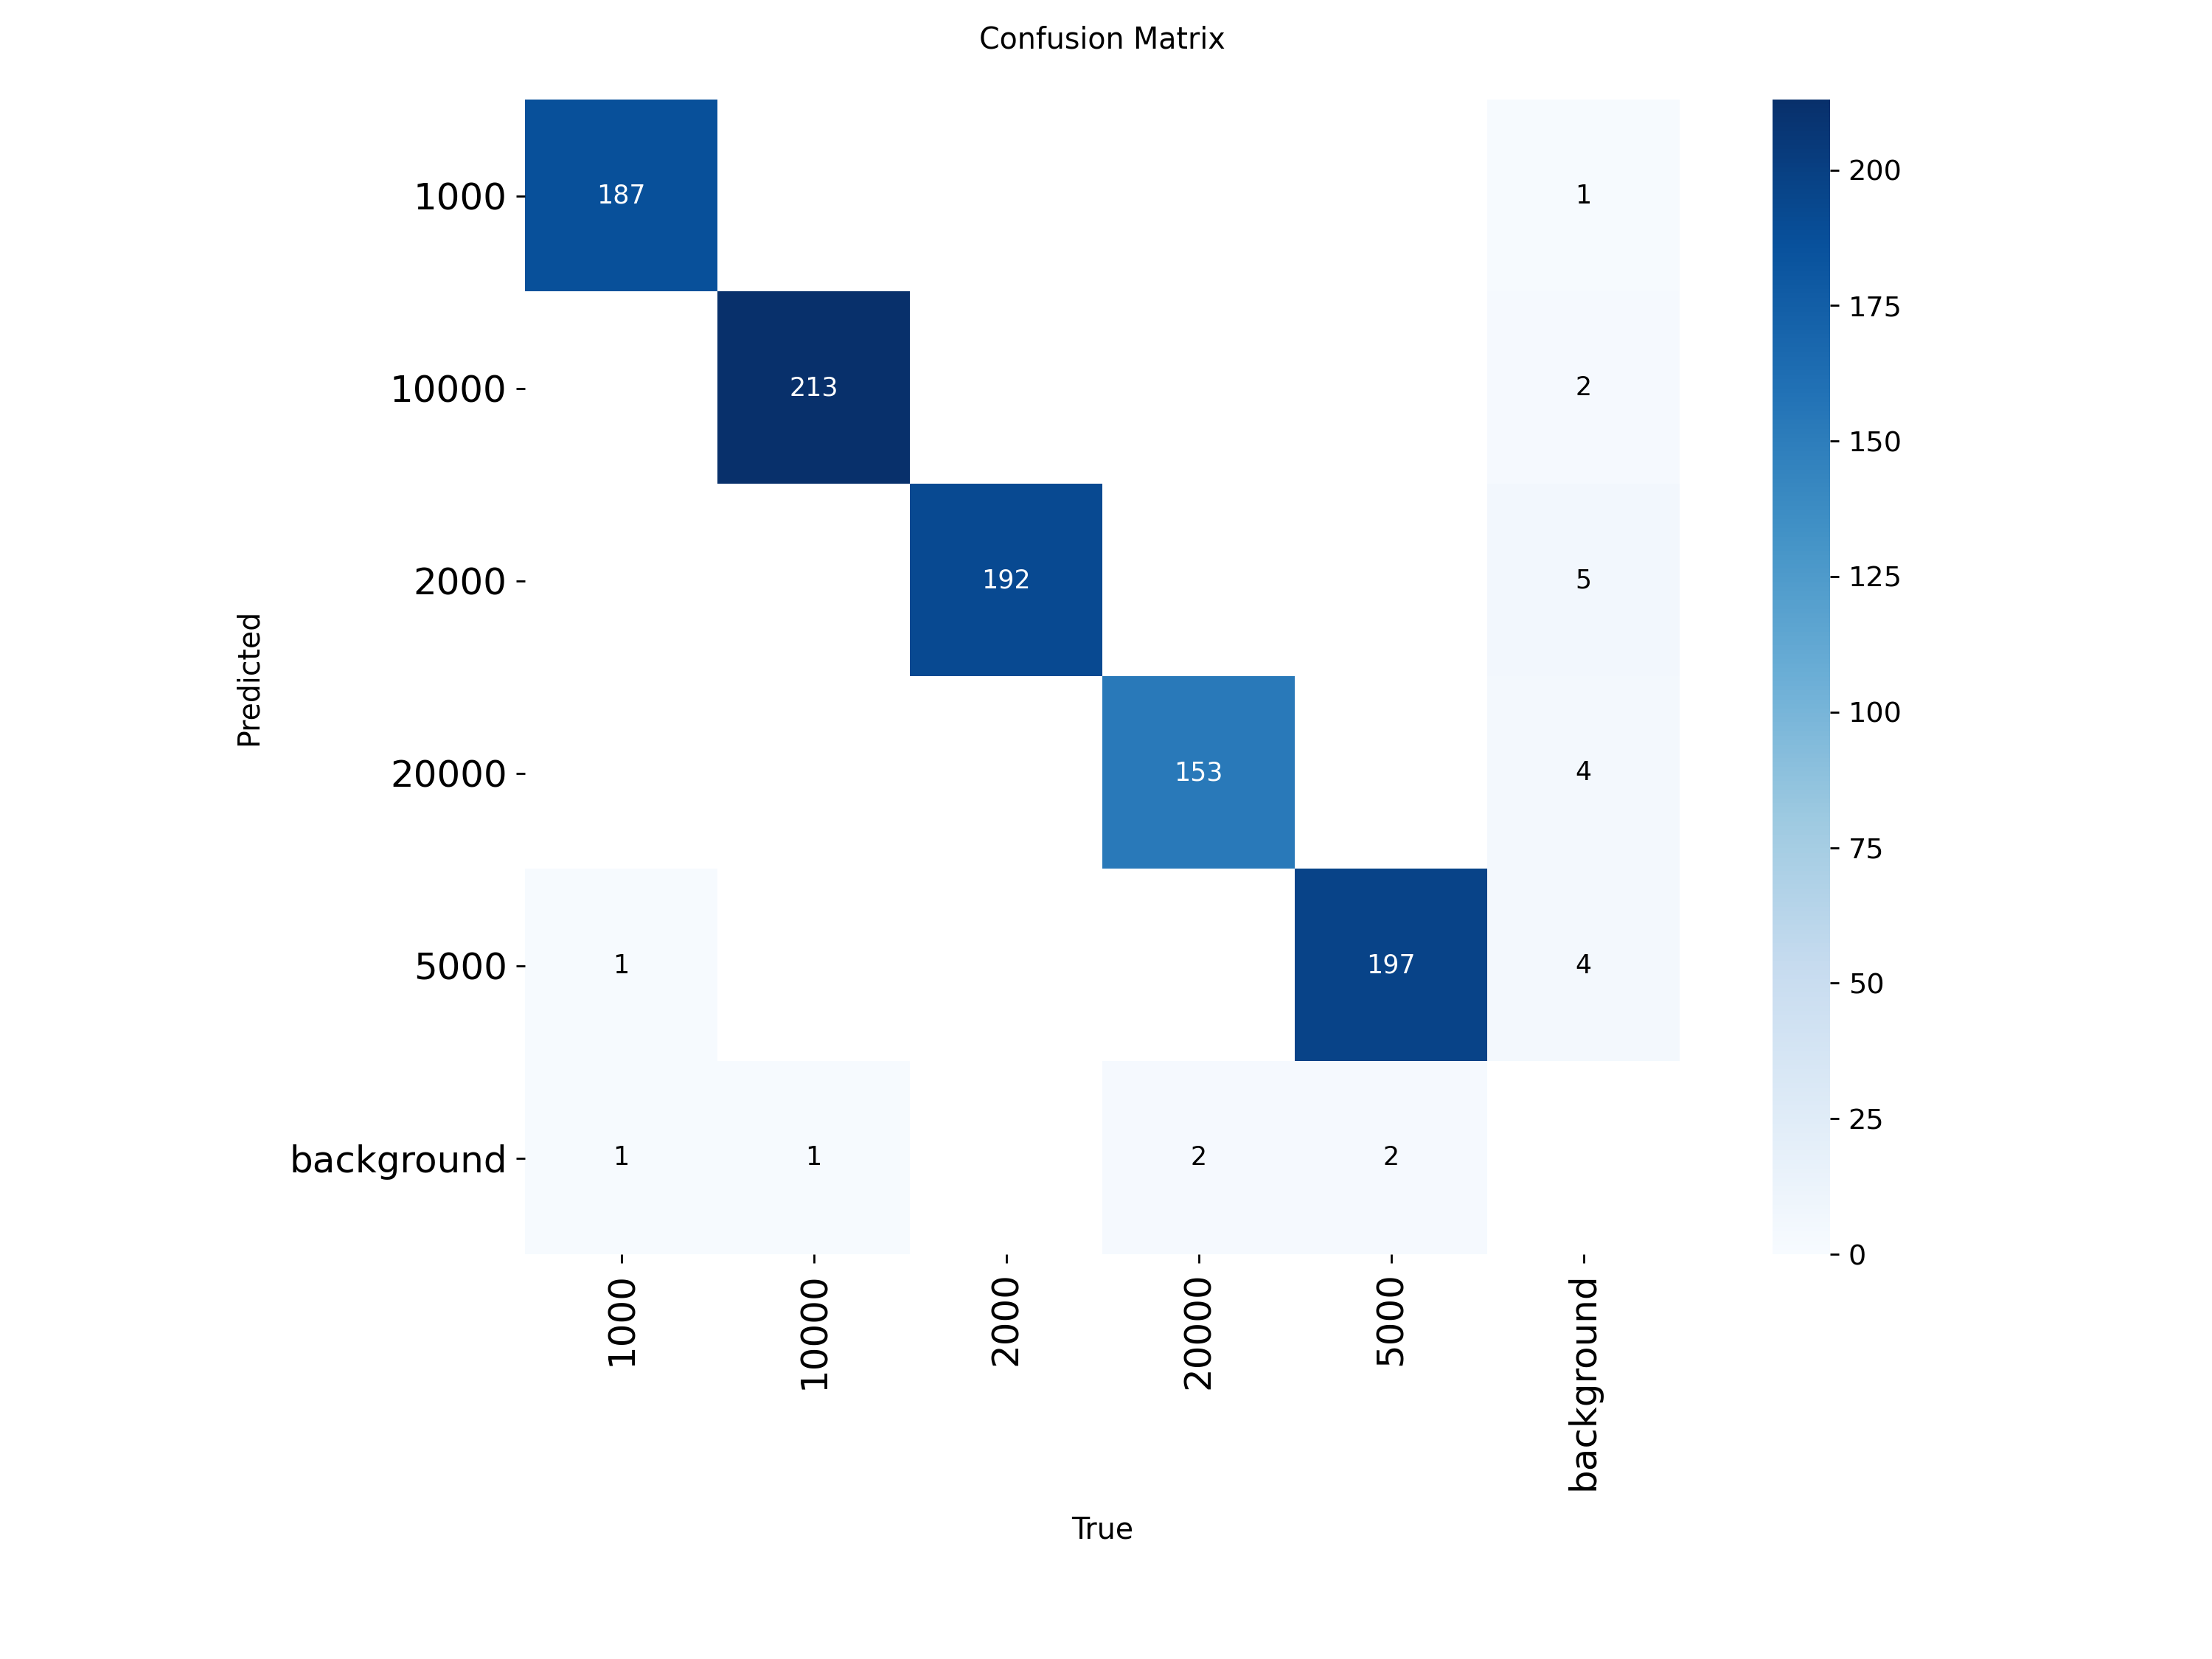
\includegraphics[width=0.8\textwidth]{DATASETS/runs/detect/train/confusion_matrix.png}
        \caption{Matriz de Confusión.}
        \label{fig:confusion_matrix}
    \end{figure}
    \begin{figure}[H]
        \centering
        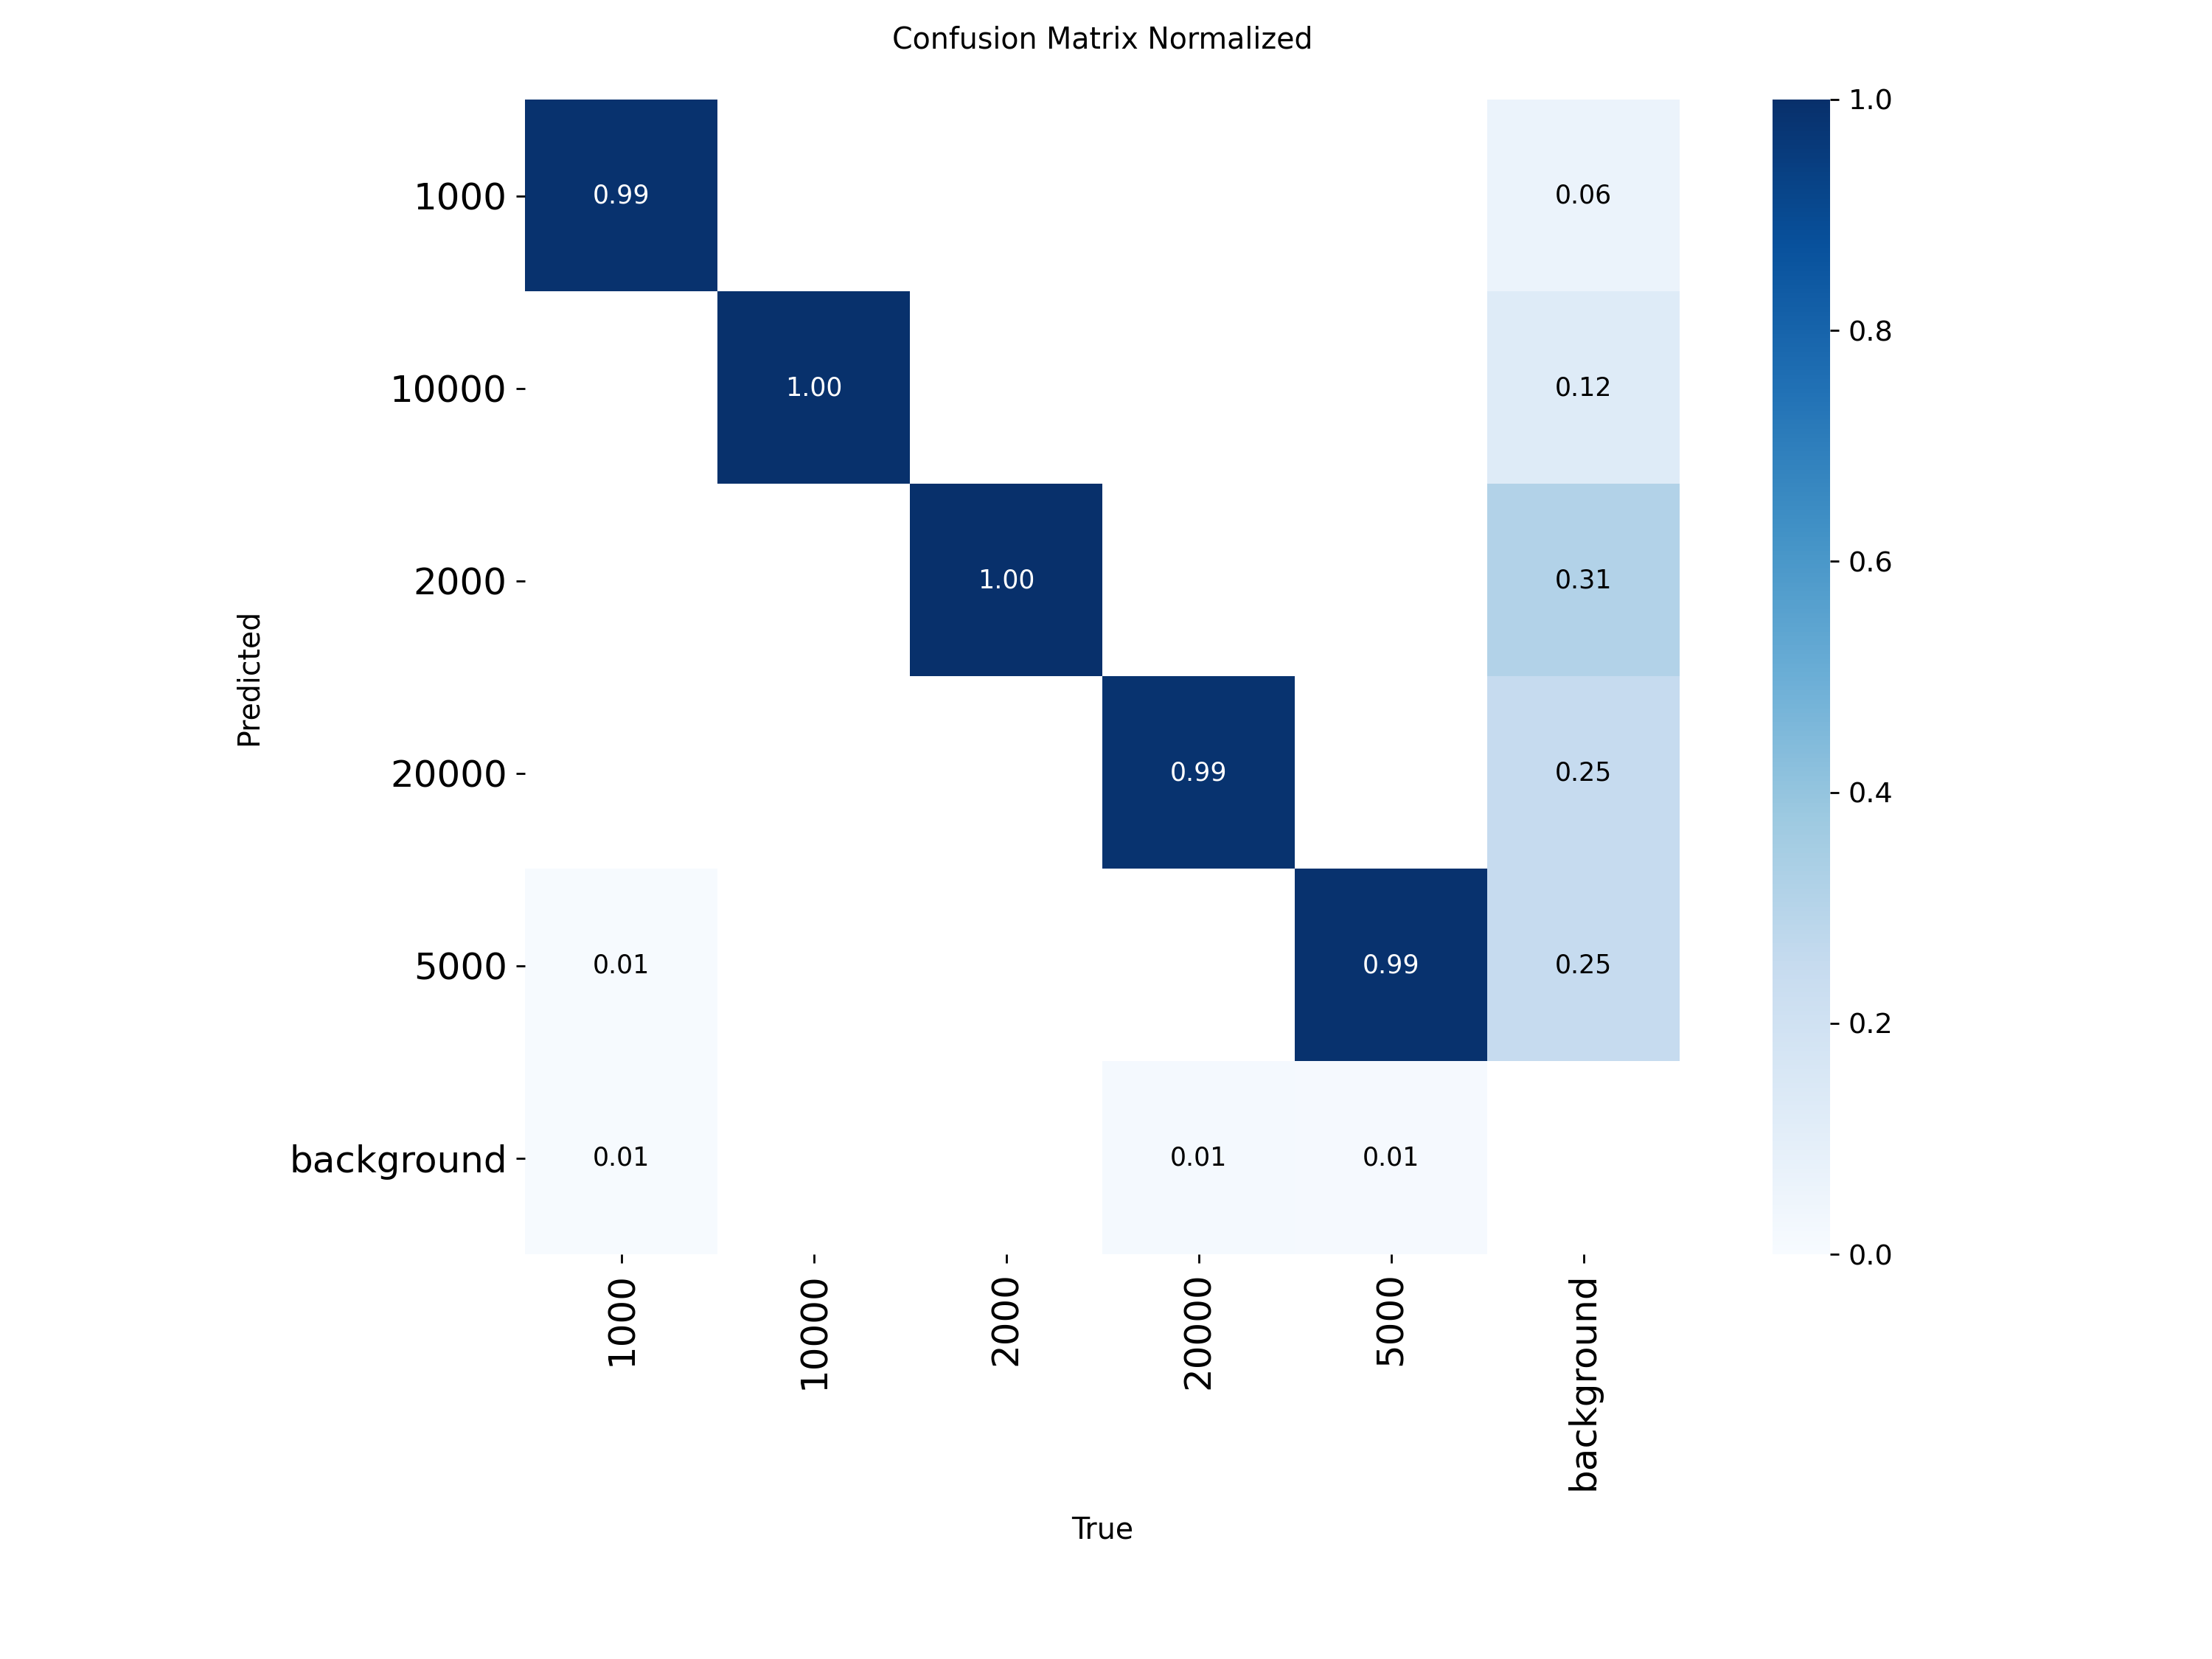
\includegraphics[width=0.8\textwidth]{DATASETS/runs/detect/train/confusion_matrix_normalized.png}
        \caption{Matriz de Confusión Normalizada.}
        \label{fig:confusion_matrix_normalized}
    \end{figure}
    La matriz de confusión (normalizada y no normalizada) muestra visualmente la proporción de verdaderos positivos, falsos positivos, verdaderos negativos y falsos negativos para cada clase. Se observa que la diagonal principal tiene valores cercanos a 1, indicando una alta tasa de aciertos.

    \item \textbf{Curvas de Precisión-Recall (PR Curve):}
    \begin{figure}[H]
        \centering
        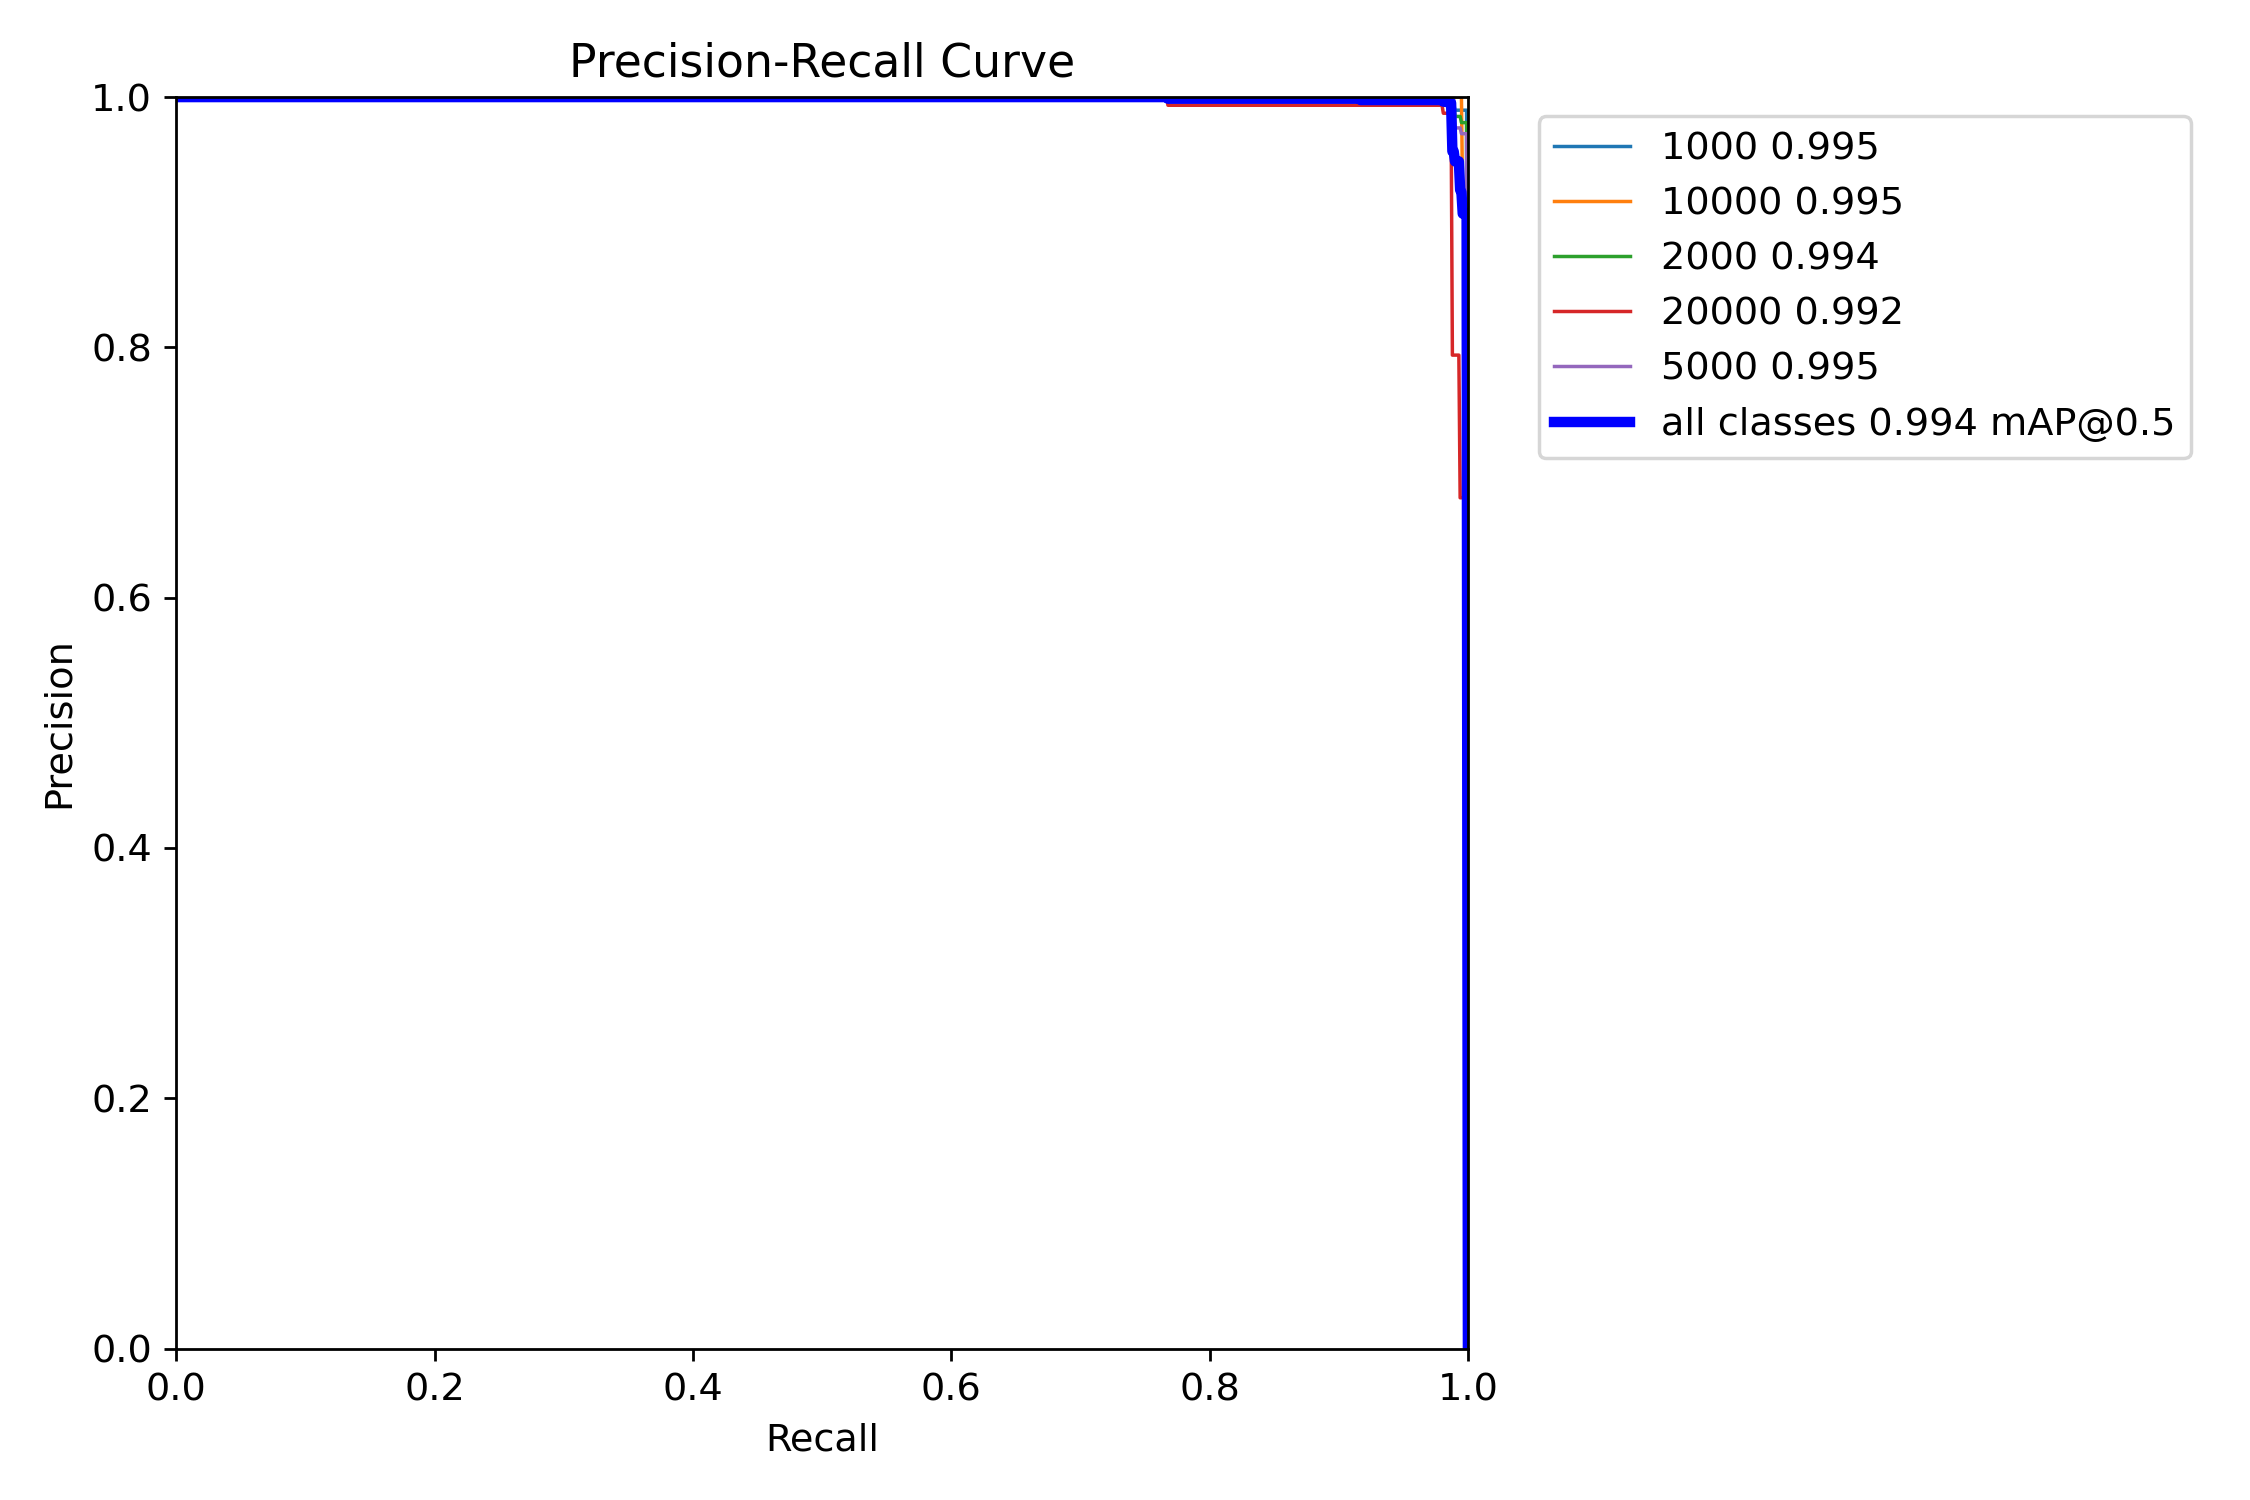
\includegraphics[width=0.8\textwidth]{DATASETS/runs/detect/train/BoxPR_curve.png}
        \caption{Curva de Precisión-Recall (PR Curve).}
        \label{fig:boxpr_curve}
    \end{figure}
    Esta curva ilustra la relación entre precisión y recall para diferentes umbrales de confianza. La curva se mantiene cerca de la esquina superior derecha, lo que indica un rendimiento excelente.

    \item \textbf{Curvas de Pérdida y Rendimiento (Loss, P, R, F1, mAP curves):}
    \begin{figure}[H]
        \centering
        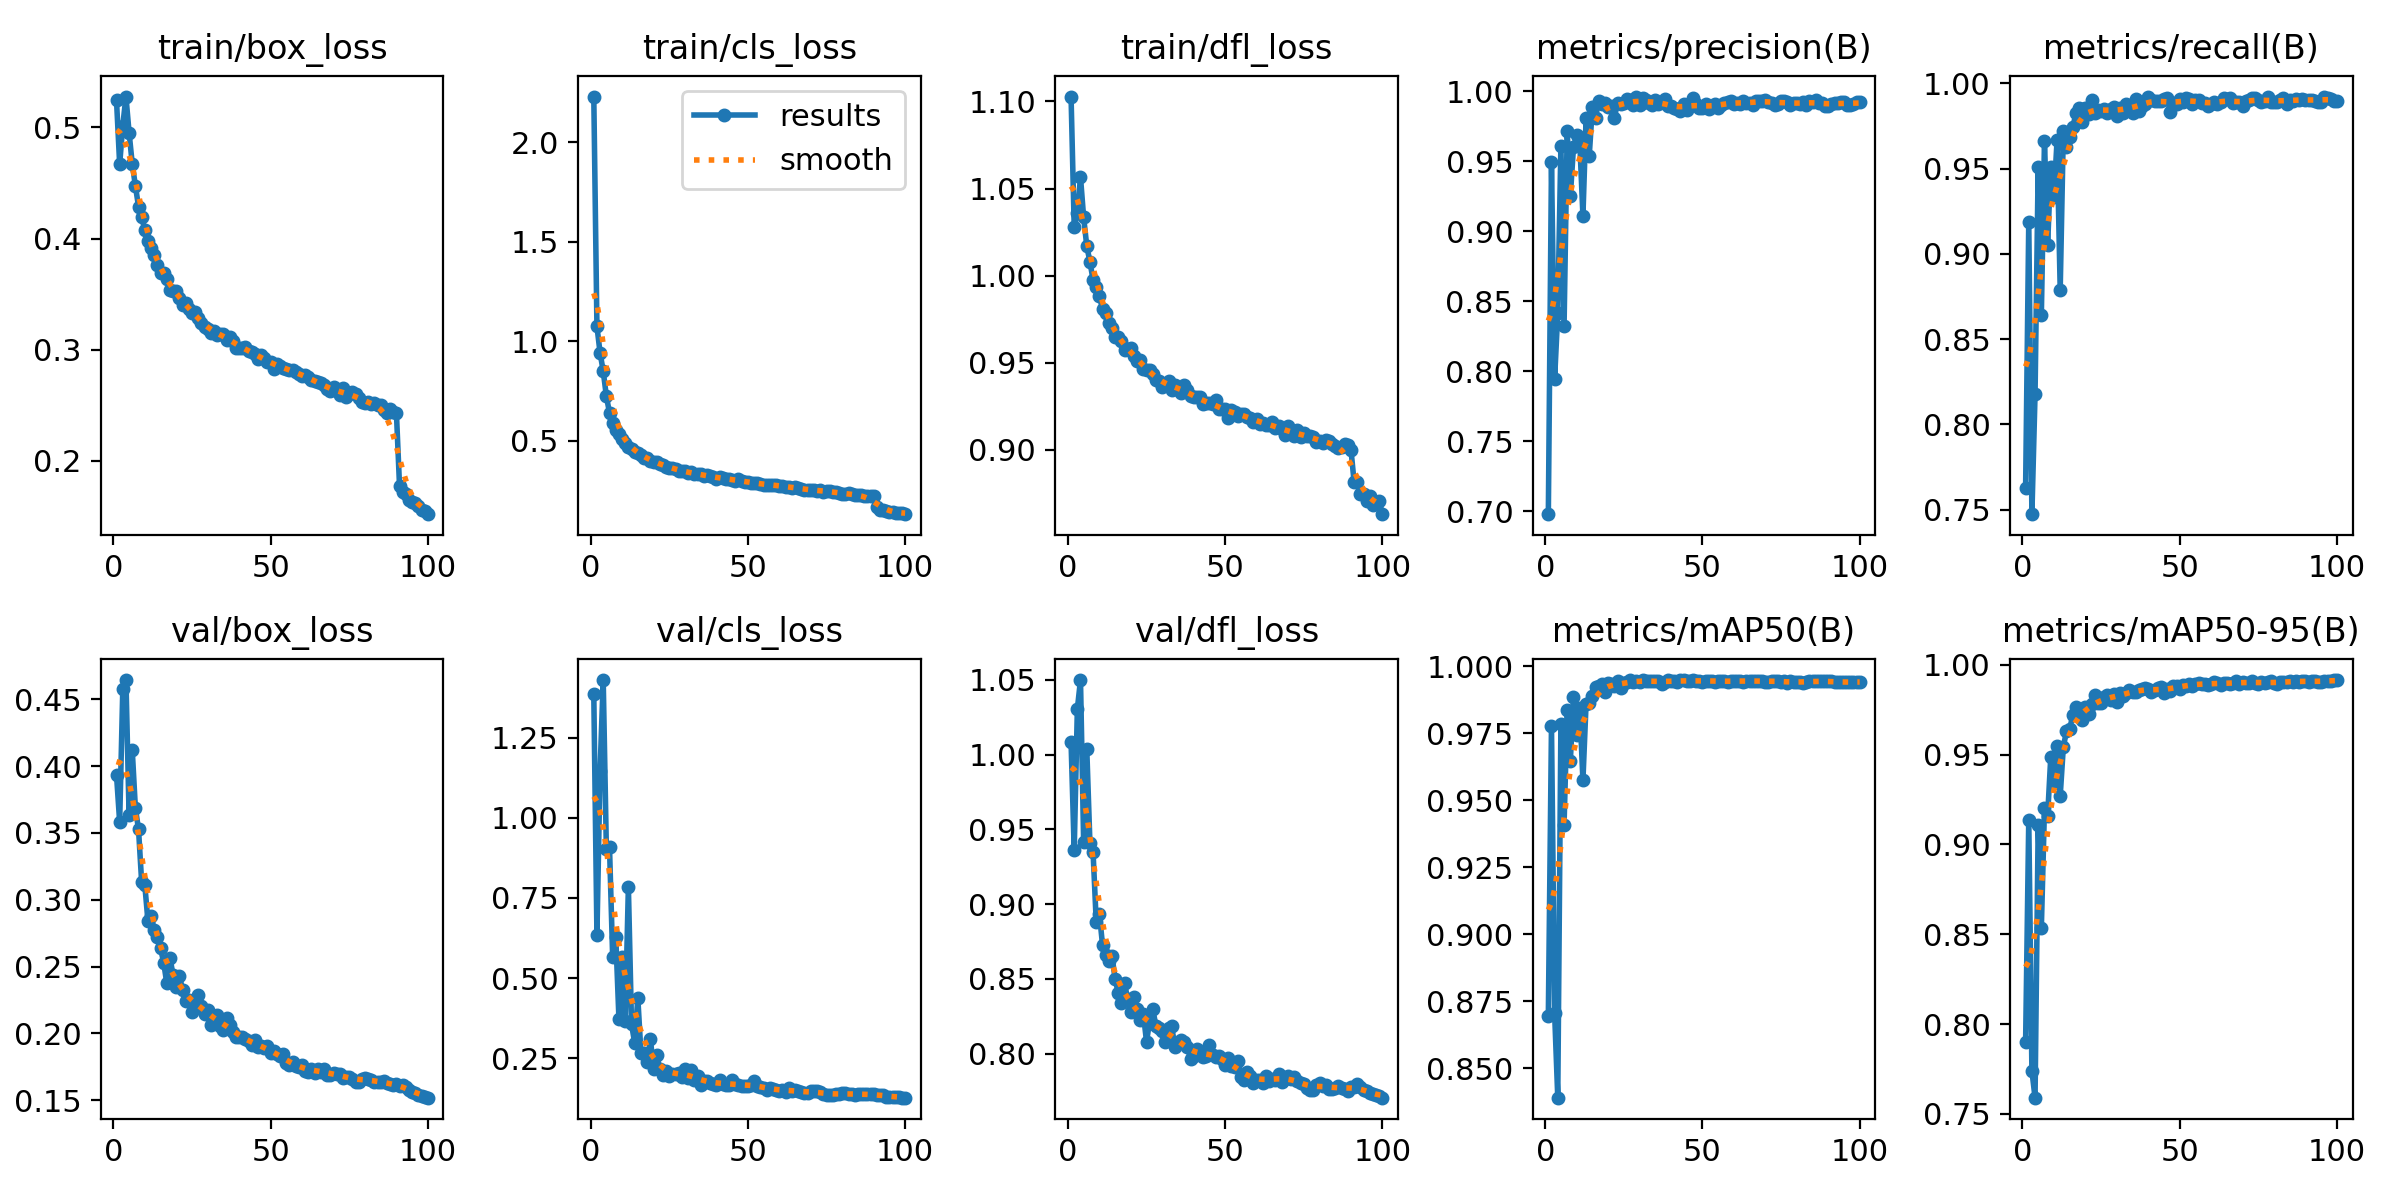
\includegraphics[width=0.8\textwidth]{DATASETS/runs/detect/train/results.png}
        \caption{Curvas de Pérdida y Rendimiento General (Loss, P, R, mAP).}
        \label{fig:results_curve}
    \end{figure}
    \begin{figure}[H]
        \centering
        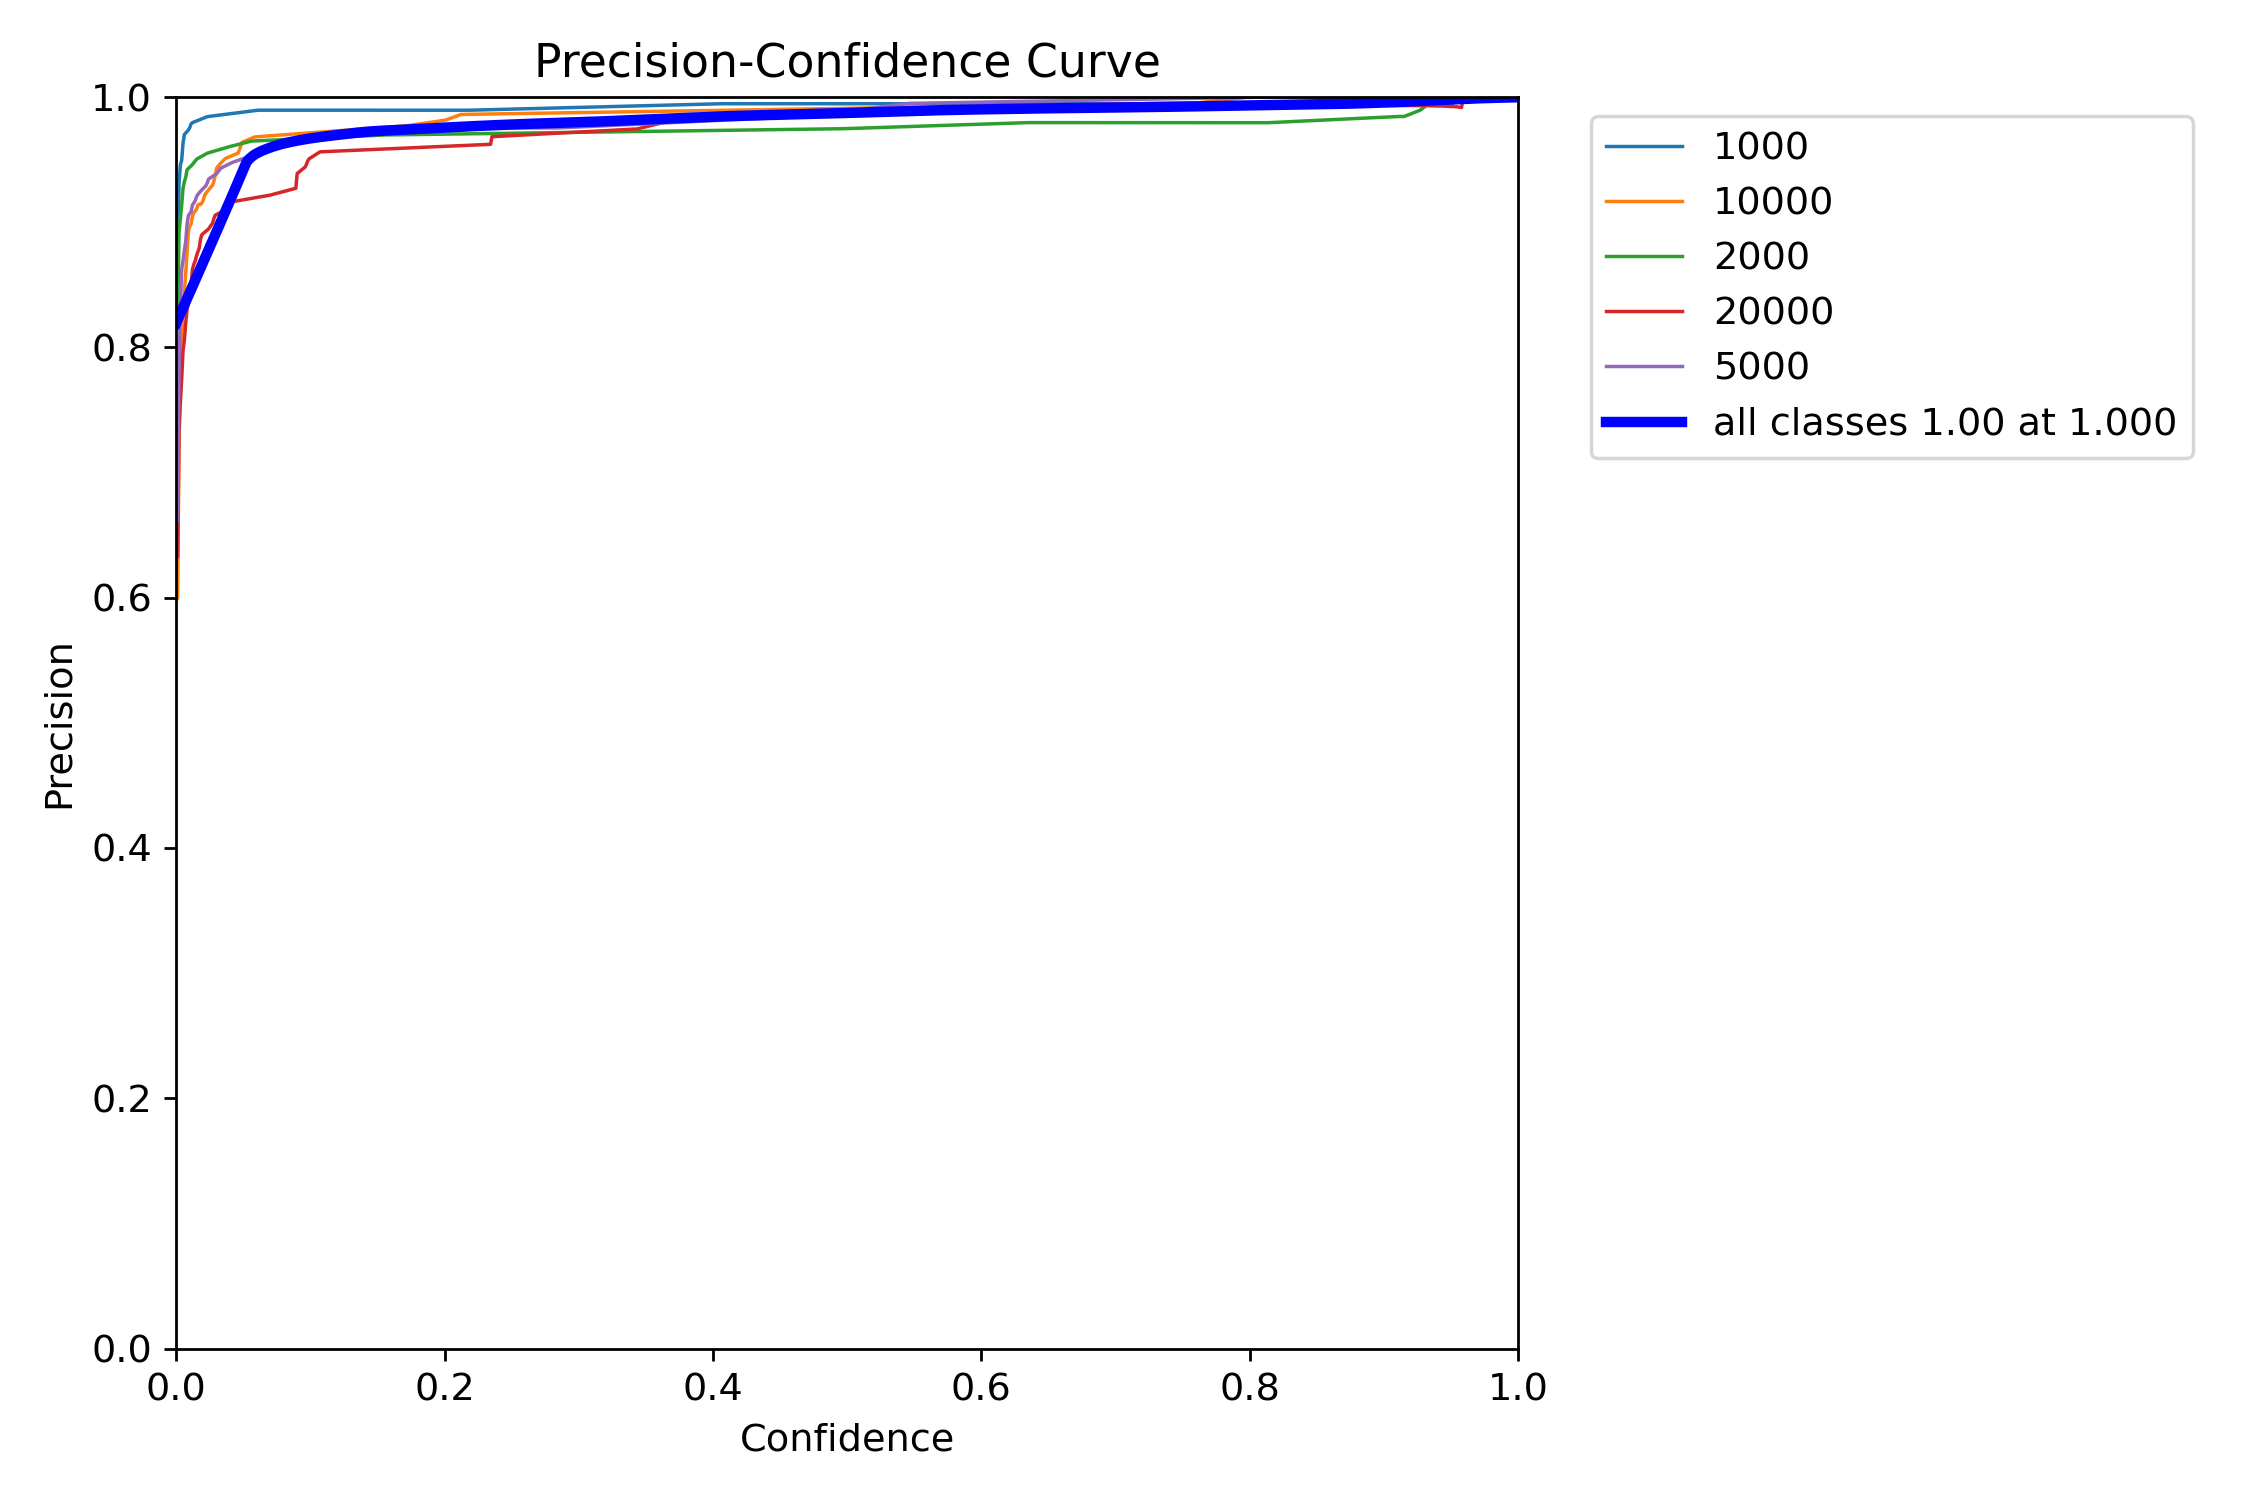
\includegraphics[width=0.8\textwidth]{DATASETS/runs/detect/train/BoxP_curve.png}
        \caption{Curva de Precisión (P Curve).}
        \label{fig:boxp_curve}
    \end{figure}
    \begin{figure}[H]
        \centering
        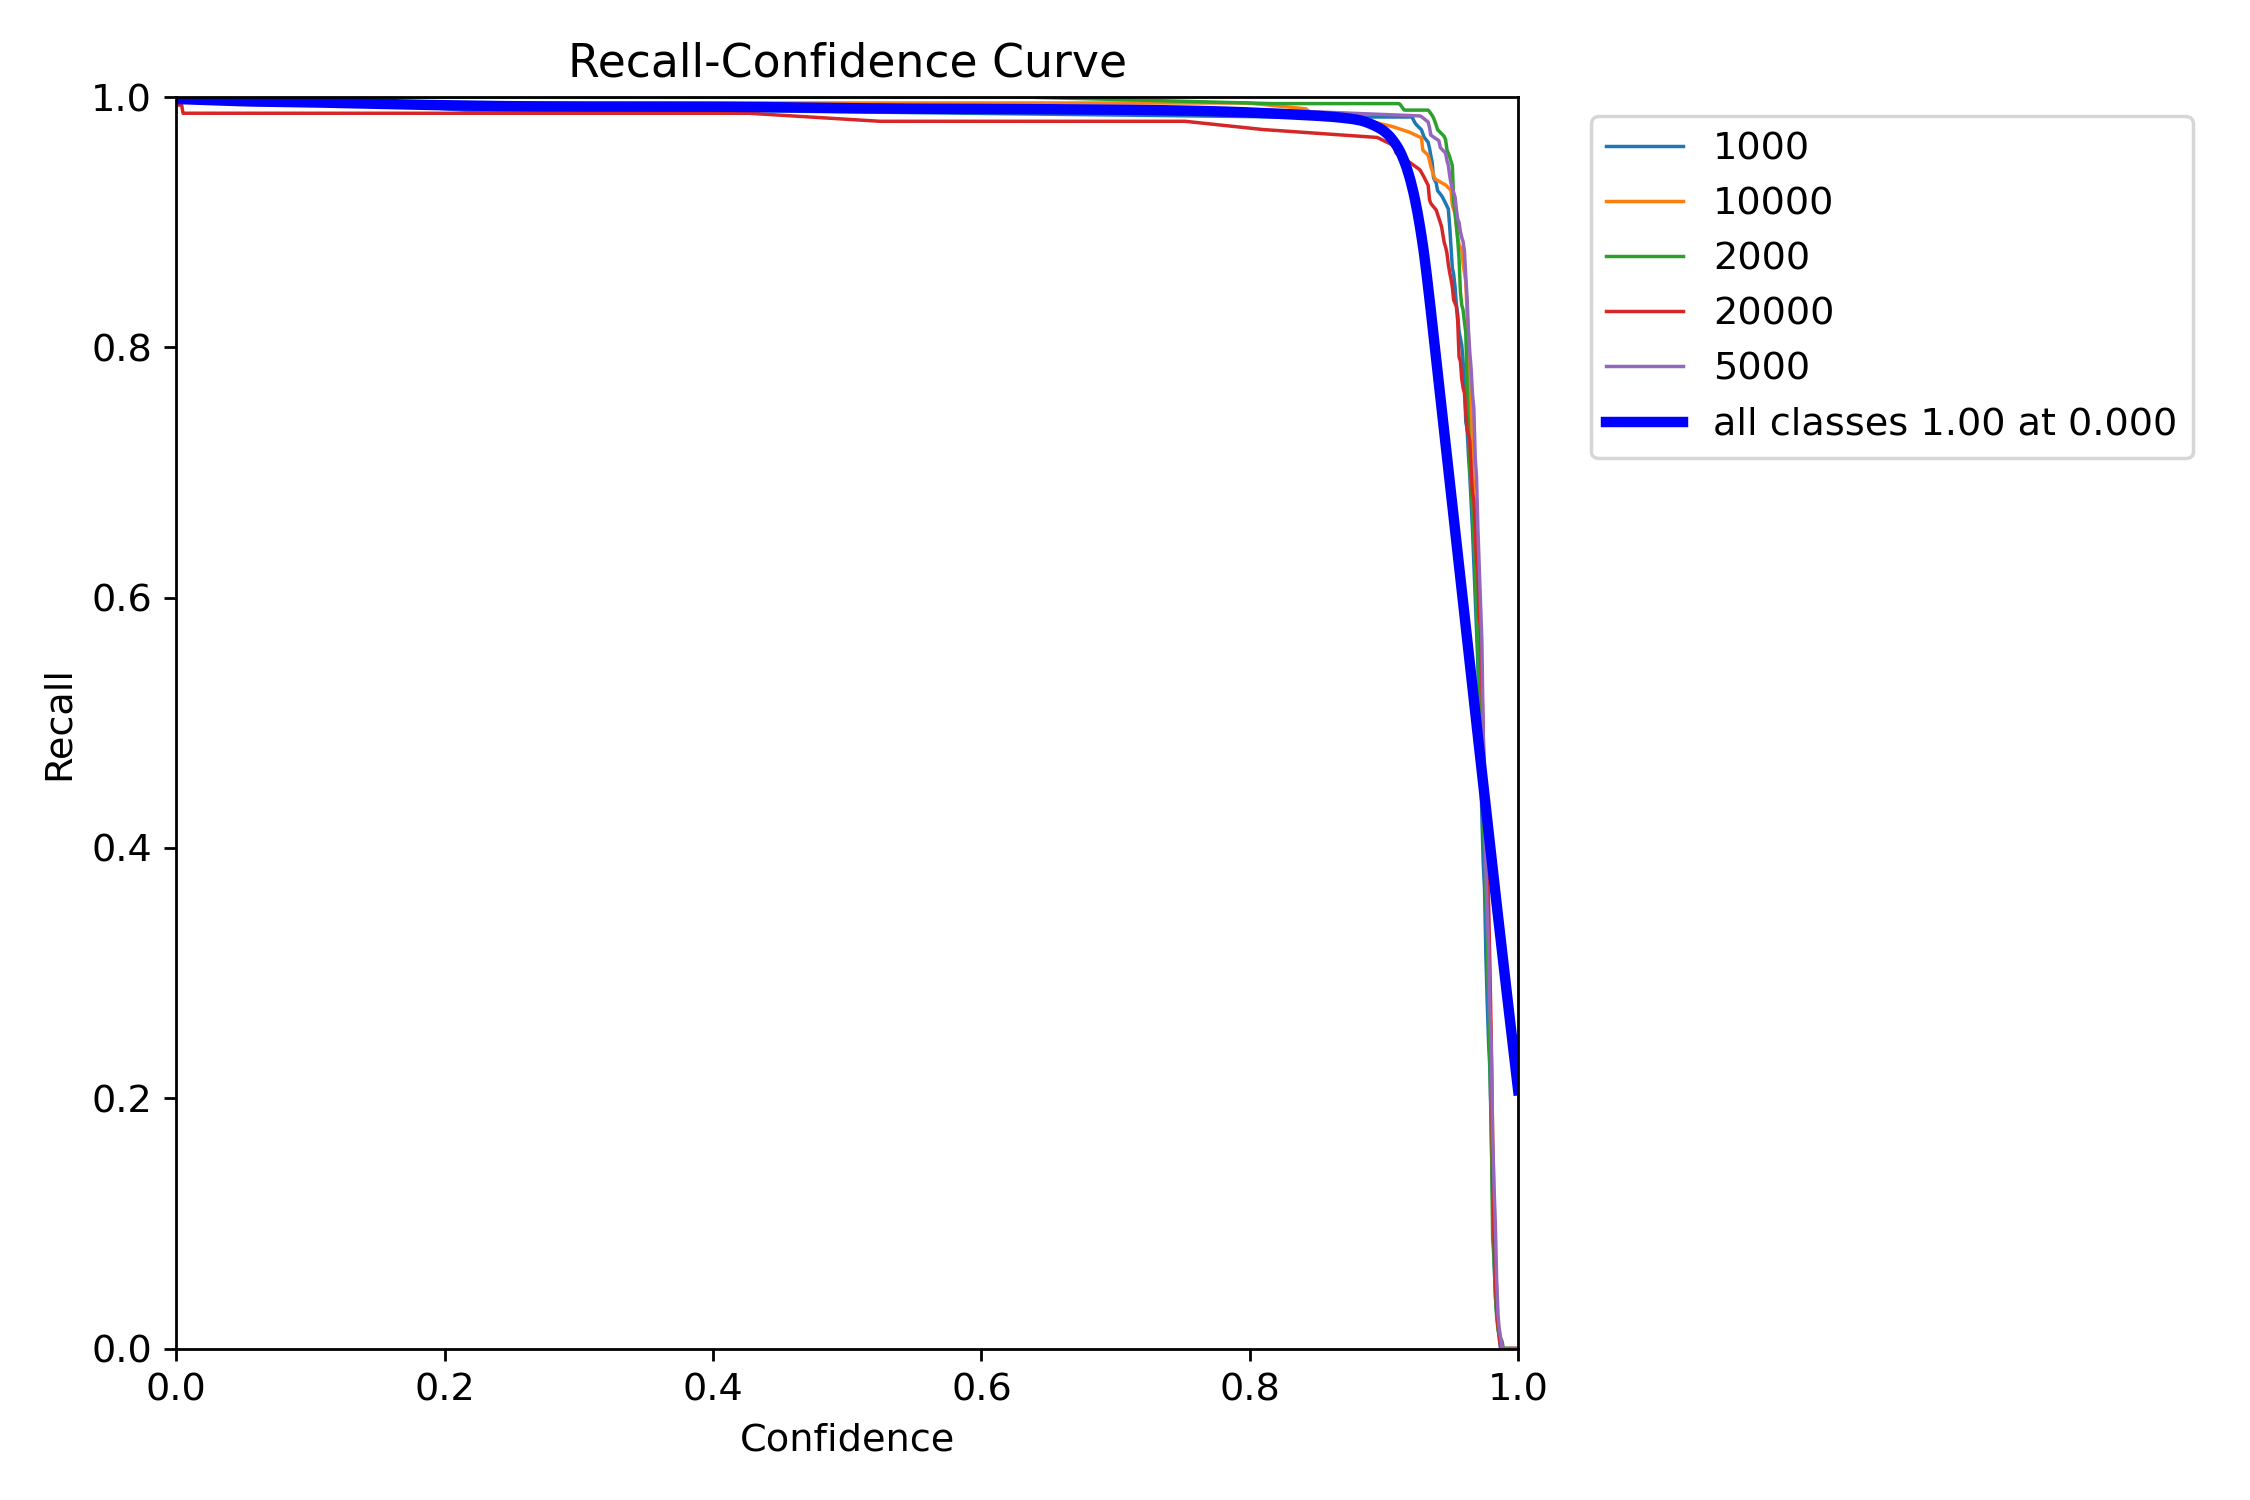
\includegraphics[width=0.8\textwidth]{DATASETS/runs/detect/train/BoxR_curve.png}
        \caption{Curva de Recall (R Curve).}
        \label{fig:boxr_curve}
    \end{figure}
    \begin{figure}[H]
        \centering
        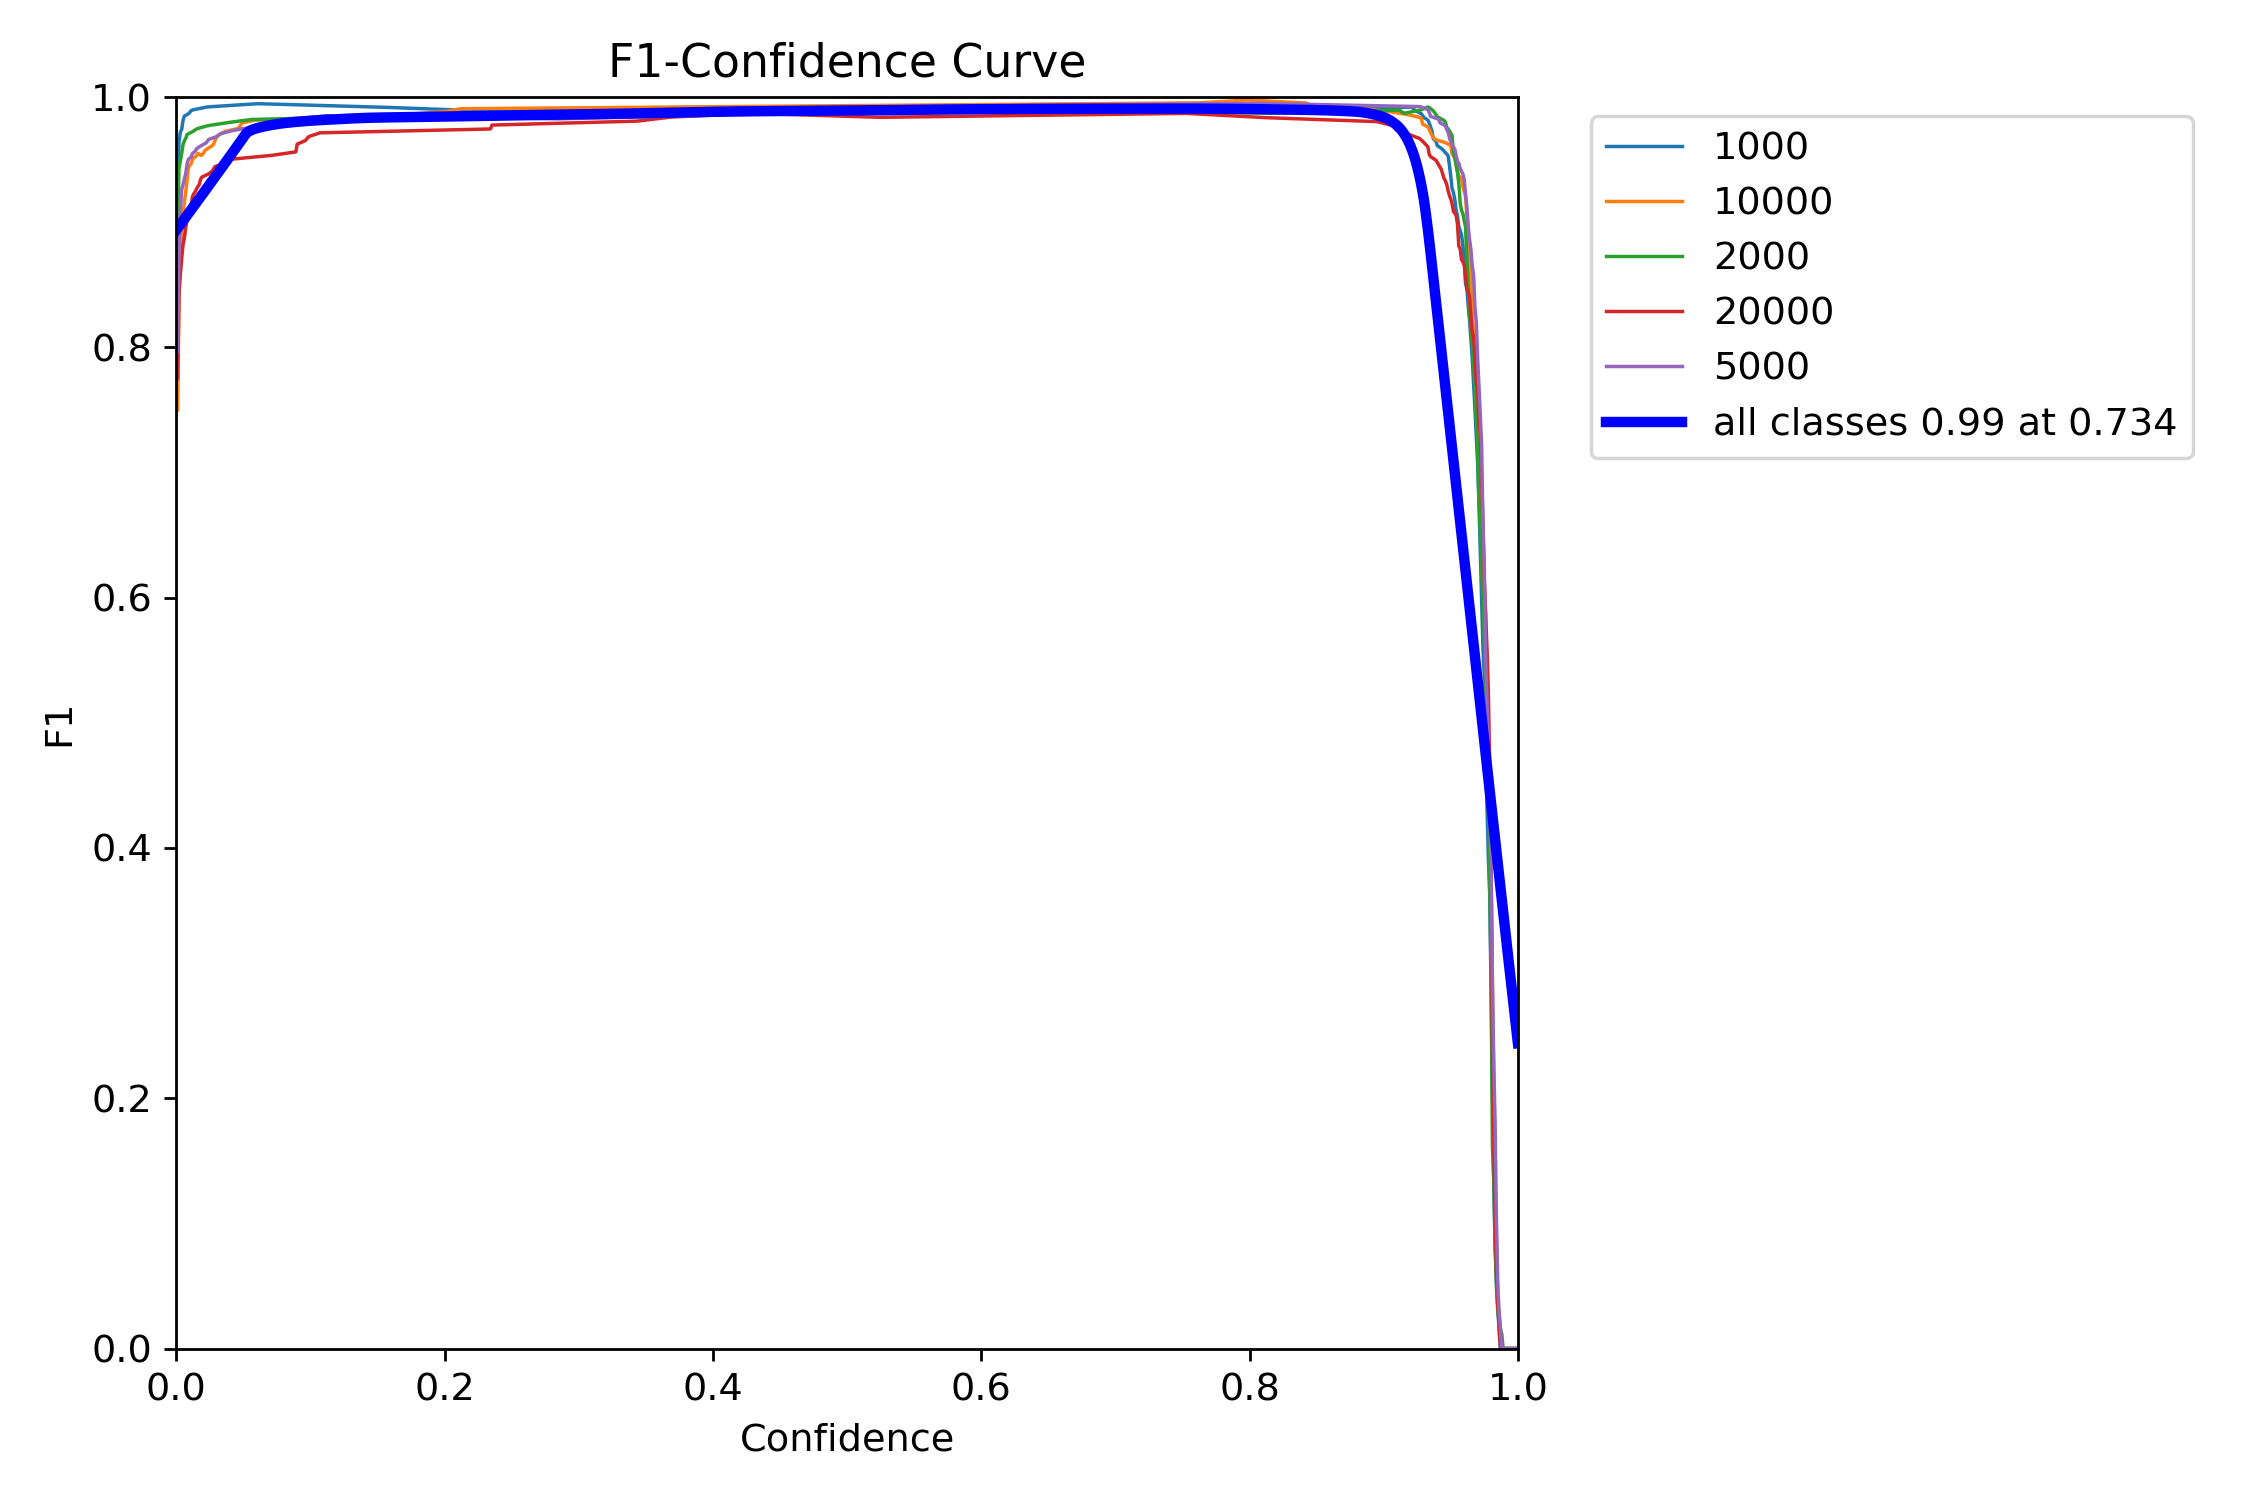
\includegraphics[width=0.8\textwidth]{DATASETS/runs/detect/train/BoxF1_curve.png}
        \caption{Curva F1-score (F1 Curve).}
        \label{fig:boxf1_curve}
    \end{figure}
    Estas imágenes consolidan la evolución de las pérdidas de entrenamiento y validación, así como las curvas de precisión, recall, F1-score y mAP a lo largo de las épocas. Se observa una estabilización y mejora continua de estas métricas hacia el final del entrenamiento, lo que corrobora la convergencia del modelo.
\end{itemize}

\textbf{Ajustes y Mejoras Concretas:}

Los resultados preliminares indican un rendimiento muy sólido del modelo, lo que sugiere que la configuración actual (YOLOv8n, 100 épocas, imgsz 640, batch 32) es efectiva para la tarea de detección.

\begin{itemize}
    \item \textbf{Validación del Diseño:} Las altas métricas de precisión, recall y mAP validan el diseño del modelo YOLOv8n para esta tarea específica. La elección de un modelo pre-entrenado y su ajuste fino con el conjunto de datos ha sido exitosa.
    \item \textbf{Necesidades de Ajuste:} Dado el excelente rendimiento, los ajustes futuros podrían centrarse en:
    \begin{itemize}
        \item \textbf{Optimización de Hiperparámetros:} Aunque el rendimiento es alto, se podría explorar un ajuste más fino de hiperparámetros como la tasa de aprendizaje (\texttt{lr0}, \texttt{lrf}), el momentum (\texttt{momentum}) o el \texttt{weight\_decay} para intentar exprimir las últimas décimas de mejora, aunque el margen es pequeño.
        \item \textbf{Análisis de Errores Específicos:} Revisar las imágenes con detecciones incorrectas (falsos positivos o falsos negativos) para identificar patrones y posibles mejoras en el preprocesamiento de datos o en la estrategia de aumento de datos.
        \item \textbf{Generalización:} Aunque las métricas de validación son buenas, se podría realizar una evaluación en un conjunto de pruebas completamente independiente para asegurar la generalización del modelo a datos no vistos.
        \item \textbf{Eficiencia Computacional:} Si la aplicación final requiere mayor velocidad o menor consumo de recursos, se podría considerar la cuantificación del modelo o la exploración de modelos más ligeros, aunque el \texttt{yolov8n} ya es una versión "nano" optimizada.
    \end{itemize}
\end{itemize}

En resumen, las pruebas iniciales confirman que el modelo ha sido entrenado con éxito, logrando un rendimiento robusto y preciso en la detección de objetos. Los ajustes futuros se enfocarán en la optimización marginal y la validación de la generalización.

\end{document}